%Time-stamp: Sat May 25 08:32:46 2013
\documentclass{beamer}
%\documentclass[serif]{beamer}

\usepackage{beamerthemesplit}
%\usepackage{mathpazo}
\usepackage{amsmath}
\usepackage{amssymb}
\usepackage{graphicx}
\usepackage{url}

\usetheme{Warsaw}
\usecolortheme{beaver}

\title[diffeqs and Euler's method]{Euler's method for solving\\
a differential equation\\
(approximately)}
\author{Math 222}
\institute{Department of Mathematics, UW - Madison}
\setlength{\parskip}{1ex plus1ex}
\begin{document}

\frame{\titlepage}

\begin{frame}{A chemical reaction}
  \centerline{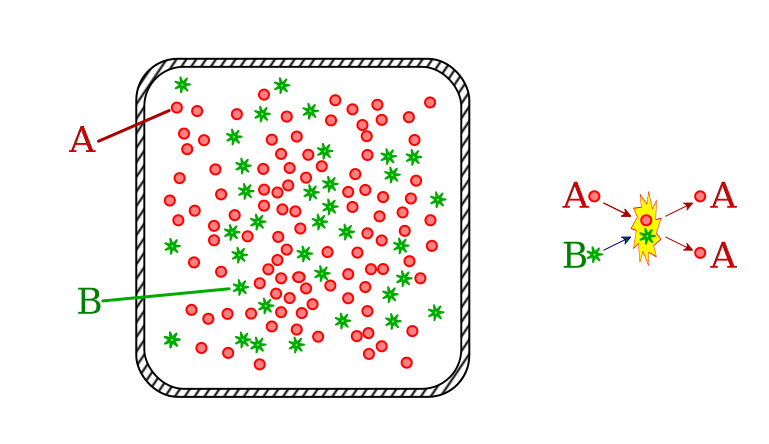
\includegraphics[width=3in]{02ABreaction.pdf}}

  A chemical reactor contains two kinds of molecules, A and B.\pause

  Whenever an A and B molecule bump into each other the B turns into an A:
  \[
  \text{A} + \text{B} \longrightarrow 2\text{A}
  \]\pause
  As the reaction proceeds, all B gets converted to A.  How long does this
  take?
\end{frame}
\begin{frame}{Reaction rate for A$+$B$\longrightarrow2$A}
  The total number of molecules (A and B) stays constant.\pause

  Let's call $x(t)$ the fraction of all molecules that at
  time $t$ are of type A:
  \[
  \textcolor{red}{x(t)} = \frac{\text{amount of A}}
  {\text{amount of A} + \text{amount of B}}
  \]\pause

  Then \textcolor{red}{$0\leq x(t) \leq 1$}, and the fraction of all
  molecules in the reactor which (at time $t$) are of type B is
  \textcolor{red}{$1-x(t)$}.\pause

  Every time a reaction takes place, the ratio $x(t)$ increases, so
  \[
  \frac{dx} {dt} \text{ is proportional to the reaction rate.}
  \]
\end{frame}

\begin{frame}{Reaction rate for A$+$B$\longrightarrow2$A}
  ``Chemistry'' tells us that
  \begin{align*}
    \frac{dx} {dt}
    &= K\cdot \textcolor{blue}{\text{amount of A}}\cdot
    \textcolor{red}{\text{amount of B}} \\
    &= K \textcolor{blue}{x}\textcolor{red}{(1-x)}.
  \end{align*}\pause
  $K$ is a proportionality constant, which depends on the particular kind
  of molecules A and B in this reaction.  You would have to measure it to
  find its value.\pause
%%%   \scriptsize
%%% 
%%%   The law of \textbf{Mass-Action} says that the rate of change of the
%%%   concentrations $[A]$ and $[B]$ of A and B molecules is given by
%%%   \[
%%%   \frac{d[A]}{dt} = k \cdot [A] \cdot [B]
%%%   \]
%%%   for some constant $k$ (the reaction rate constant).  Since
%%%   $x= \frac{[A]}{[A] + [B]}$ this implies the equation
%%%   $\frac{dx}{dt} = Kx(1-x)$ for $x(t)$ which
%%%   we're using this hour.\pause
%%% 
%%% 
%%% 
%%%   \normalsize
%%% 
  This is a calculus class, so \textcolor{magenta}{let's assume $K=1$.}
\end{frame}

\begin{frame}{Solving $\frac{dx} {dt} = x(1-x)$}
  We have to solve the diffeq
  \[
  \frac{dx} {dt} = x(1-x).
  \]
  The solution will have an arbitrary constant (``$C$'').  If we know what
  $x(0)$ is then we can compute $C$.\pause

  So (as an example) let's try to solve the following problem:\pause

  Suppose the tank initially holds 2\% A and 98\% B,\pause \hfill
  \textcolor{red}{$x(0)=0.02$}\pause\\
  Then what is the fraction of A molecules at time
  $t$?\hfill\pause \textcolor{red}{$x(t) = $?} 

\end{frame}

\begin{frame}{Summary of the problem}
  We are going to solve an \textcolor{blue}{initial value problem:}\pause

  Find $x(t)$ if you know 
  \[
  \underbrace{\frac{dx} {dt} = x(1-x)}_{\text{diffeq, holds for }t>0}
  \quad\text{and}\quad
  \underbrace{x(0)=0.02}_{\text{initial value}}
  \]\pause
  The solution is
  \[
  x(t) = \frac{1} {1+49e^{-t}}.
  \]
  (to be explained later this hour).
\end{frame}
\begin{frame}{Leonhard ``$e^{\pi i} + 1 = 0$'' Euler\hfill (1707 - 1783)}\centering
  \includegraphics[scale=0.5]{Euler_9.jpeg}

\end{frame}
\begin{frame}{Solving $\frac{dx} {dt} = x(1-x)$}
  Euler's idea:\pause

  I can't solve the equation because I don't know what
  $\frac{dx} {dt}$ is.  So pick a small number $h>0$ and say that
  \[
  \frac{dx} {dt} \approx \frac{x(t+h) - x(t)} {h}.
  \]\pause
  The diffeq then becomes
  \[
  \frac{x(t+h) - x(t)} {h} \approx x(t)(1-x(t)).
  \]
  \pause

  If you know $x(t)$ and $h$ then you can solve this equation for $x(t+h)$.
\end{frame}

\begin{frame}{Solving $\frac{dx} {dt} = x(1-x)$}
  \[
  \frac{ \textcolor{red}{x(t+h)} - \textcolor{blue}{x(t)} } {h}
  \approx \textcolor{blue}{x(t)(1-x(t))}.
  \]
  has as solution
  \[
  \textcolor{red}{x(t+h)}\approx
  \textcolor{blue}{x(t)} + h\cdot \textcolor{blue}{x(t)(1-x(t))}.
  \]
  \pause

  \textbf{Example ($t=0$): }
  If we know $x(0)$, then this equation allows us to compute $x(0+h) =
  \textcolor{red}{x(h)}$.\pause

  \textbf{Example ($t=h$): }
  Knowing $x(h)$ you can find $x(h+h) = \textcolor{red}{x(2h)}$\pause,

  And then $x(2h+h) = \textcolor{red}{x(3h)}$, \pause
  $x(3h+h) = \textcolor{red}{x(4h)}$, etc.\ldots
\end{frame}

\begin{frame}{Euler's (approximate) solution}
  Pick a small number $h>0$, and compute
  \begin{center}
    \begin{tabular}[h]{rcl}
      $\textcolor{red}{x(h)}$& $=$ & $x(0) + h\cdot
      x(0)[1-x(0)]$\pause\\
      &$\searrow$\\
      $\textcolor{blue}{x(2h)}$&$=$ & $ \textcolor{red}{x(h)} + h\cdot
      \textcolor{red}{x(h)}[1-\textcolor{red}{x(h)}]$\pause\\ 
      &$\searrow$\\
      $\textcolor{orange}{x(3h)}$&$=$ & $\textcolor{blue}{x(2h)} + h\cdot
      \textcolor{blue}{x(2h)}[1-\textcolor{blue}{x(2h)}]$\pause\\ 
      &$\searrow$\\
      $\textcolor{olive}{x(4h)}$&$=$ & $ \textcolor{orange}{x(3h)} + h\cdot
      \textcolor{orange}{x(3h)}[1-\textcolor{orange}{x(3h)}]$\pause\\ 
      &$\vdots$
    \end{tabular}
  \end{center}
  \pause%
  Now let's choose $h=0.2$ and $x(0) = 0.02$, and compute $x(0.2)$,
  $x(0.4)$, $x(0.6)$, $x(0.8)$, $x(1.0)$,  \ldots
\end{frame}

\begin{frame}{Doing the calculations}
  Doing all these calculations is a drag of course.  How did Euler do this?
  By hand!! (and with a lot of patience).\pause

  How do we do this in the 21st century?  With a computer.\pause

  For more complicated diffeqs one should learn to program a computer, but
  for the example we've been looking at you can get Excel (or some other
  spreadsheet program like Open Office) to compute and plot the solutions.
\end{frame}
\begin{frame}{What the spreadsheet computed\\
  {\tiny Here are the numbers, and graphs.  The exact solution is $x(t) =
  1/(1+49e^{-t})$.}}
  \includegraphics[width=0.3\textwidth]{euler-output.pdf}\hfill
  \includegraphics[width=0.5\textwidth]{euler-graphs.pdf}
\end{frame}
\begin{frame}{Point and click on-line diffeq solver}
  There are several graphical on-line solvers for differential
  equations.  If you go to this web page:

  \textcolor{red}{
  \url{http://virtualmathmuseum.org/ODE/1o1d-MassAction}}

  you can see graphs of the solution to our equation
  $\frac{dx}{dt} = x(1-x)$.
\end{frame}
\end{document}
